\documentclass[11pt, oneside]{article}   	% use "amsart" instead of "article" for AMSLaTeX format
\usepackage{geometry}                		% See geometry.pdf to learn the layout options. There are lots.
\geometry{letterpaper}                   		% ... or a4paper or a5paper or ...
%\geometry{landscape}                		% Activate for rotated page geometry
%\usepackage[parfill]{parskip}    		% Activate to begin paragraphs with an empty line rather than an indent
\usepackage{graphicx}				% Use pdf, png, jpg, or eps§ with pdflatex; use eps in DVI mode
								% TeX will automatically convert eps --> pdf in pdflatex
\graphicspath{ {assets/} }								
\usepackage{amssymb}
\usepackage{amsmath}
\usepackage{float}
\usepackage{hyperref}

%SetFonts

%SetFonts


\title{Dominion: A Board Game Breakdown}
\author{Bryan Alcorn}
\date{Stats 157}							% Activate to display a given date or no date

\begin{document}

\maketitle

\section{Dominion}

You are a monarch, like your parents before you, a ruler of a small pleasant kingdom of rivers and evergreens.
Unlike your parents, however, you have hopes and dreams!
You want a bigger and more pleasant kingdom, with more rivers and a wider variety of trees.
You want a Dominion! In all directions lie fiefs, freeholds, and feodums.
All are small bits of land, controlled by petty lords and verging on anarchy.
You will bring civilization to these people, uniting them under your banner.

\section{Motivation}

I have always wanted to try and apply statistics to a game, blending together my interests for computer science and statistics. My roommate recently introduced me to the game and we are currently battling over who can end the semester on top of the leaderboard. We are currently tied and I am hoping this game will change that. 

Furthermore, I want to try and play smarter. I want to see if it is possible for me to get real world insights out of testing a game that I built. Not only do I have to build a working game of dominion, but I have to design it in a way such that it can be played automatically so that I can test it. 

\section{Rules}

\subsection{Setup}

The game starts by selecting the cards to be used for the game. From the 26 possible kingdom cards, you will choose any combination of 10. 

Each player receives 7 copper and 3 estates as a starting deck.

\subsection{Gameplay}

During each turn, you draw 5 cards from your deck, after you play a card it is labeled as played. At the end of every hand, all those cards go into a discard. When you can no longer draw, shuffle the discard pile and make that the new deck. You should be able to always draw unless all cards are played. 

Each hand begins with 1 buy and 1 action. 


\subsection{There are four phases for a hand}

	\begin{enumerate}
 		 \item \textbf{Actions} Play an action card, follow the instructions on the card, and deduct one from your action points. 
  		 \item \textbf{Buy} a card from the board if you have enough money and deduct one from your buy points. Normally this will be just one buy per hand. 
		 \item \textbf{Cleanup} Everything in the hand, the purchased card, and the played cards go in discard
		 \item \textbf{Draw} Draw again to 5. You should have 5 in your hand before you play in case another action card requires you to modify your hand in some way. 
	\end{enumerate}


\subsection{End}

The game ends if there are no more provinces left or three of the stockpiles are empty. The player with the most victory card count wins. 

\section{General Approach}

	\begin{enumerate}
 		 \item Build a playable version of the game in Python
		 \item Calculate some basic probabilities to get an intuition into which strategies might work best or to determine some simple tricks to play better
		 \item Modify the game so that various strategies can be played against each other with varying number of players
		 \item Build the strategies
		 \item Based on the best strategies, build an in game helper that tells you what to play so you can ask it what to play during a real game against friends.
		 \item Using the simulations, generate test data to run some statistical models on the results of the games to get insight into which cards are most effective
	\end{enumerate}


\section{Goals}

	\begin{enumerate}
 		 \item Learn about designing a game that can we can run simulations on to learn more about what actions tend to lead to victory
		 \item Test our assumptions by making different strategies and putting them against each other to see which one is better
		 \item Determine which cards give us the most value during a game
	\end{enumerate}


\section{Game Design}

The game is built using object oriented programming in Python. The game is broken down into three main operational files

	\begin{itemize}
  		\item \textbf{\textit{player.py}} - The player controls everything relating to their deck and hand. They draw, discard, play, and win. 
  		\item \textbf{\textit{gameBoard.py}} - The board manages everything a player has to interact with. It contains the gold, the stockpiles, and methods to interact with the board. The board has a subclass called \textbf{\textit{Cards}} and each card can be played by a player on a game board. 
		\item \textbf{\textit{play.py}} - Play manages the logic of the game. This is where you select the initial cards to play with, it checks to make sure money >= cost of a card when buying, and it also manages every turn until someone wins.  Strategies will also be added onto this to made the decisions then their player comes up. Instead of asking the player what to do, the strategies will take care of the buy or play decisions. 
	\end{itemize}
	
From there, \textbf{\textit{strategies.py}} was added on as a way to attach different strategies to \textbf{\textit{play.py}} and \textbf{\textit{models.py}} is used to do tests and calculate probabilities. 

\section{Command Line Interface}

The game is playable through the command line with commands to buy, play, or end the turn. 

\begin{figure}[H]
\hspace*{-1.3in}
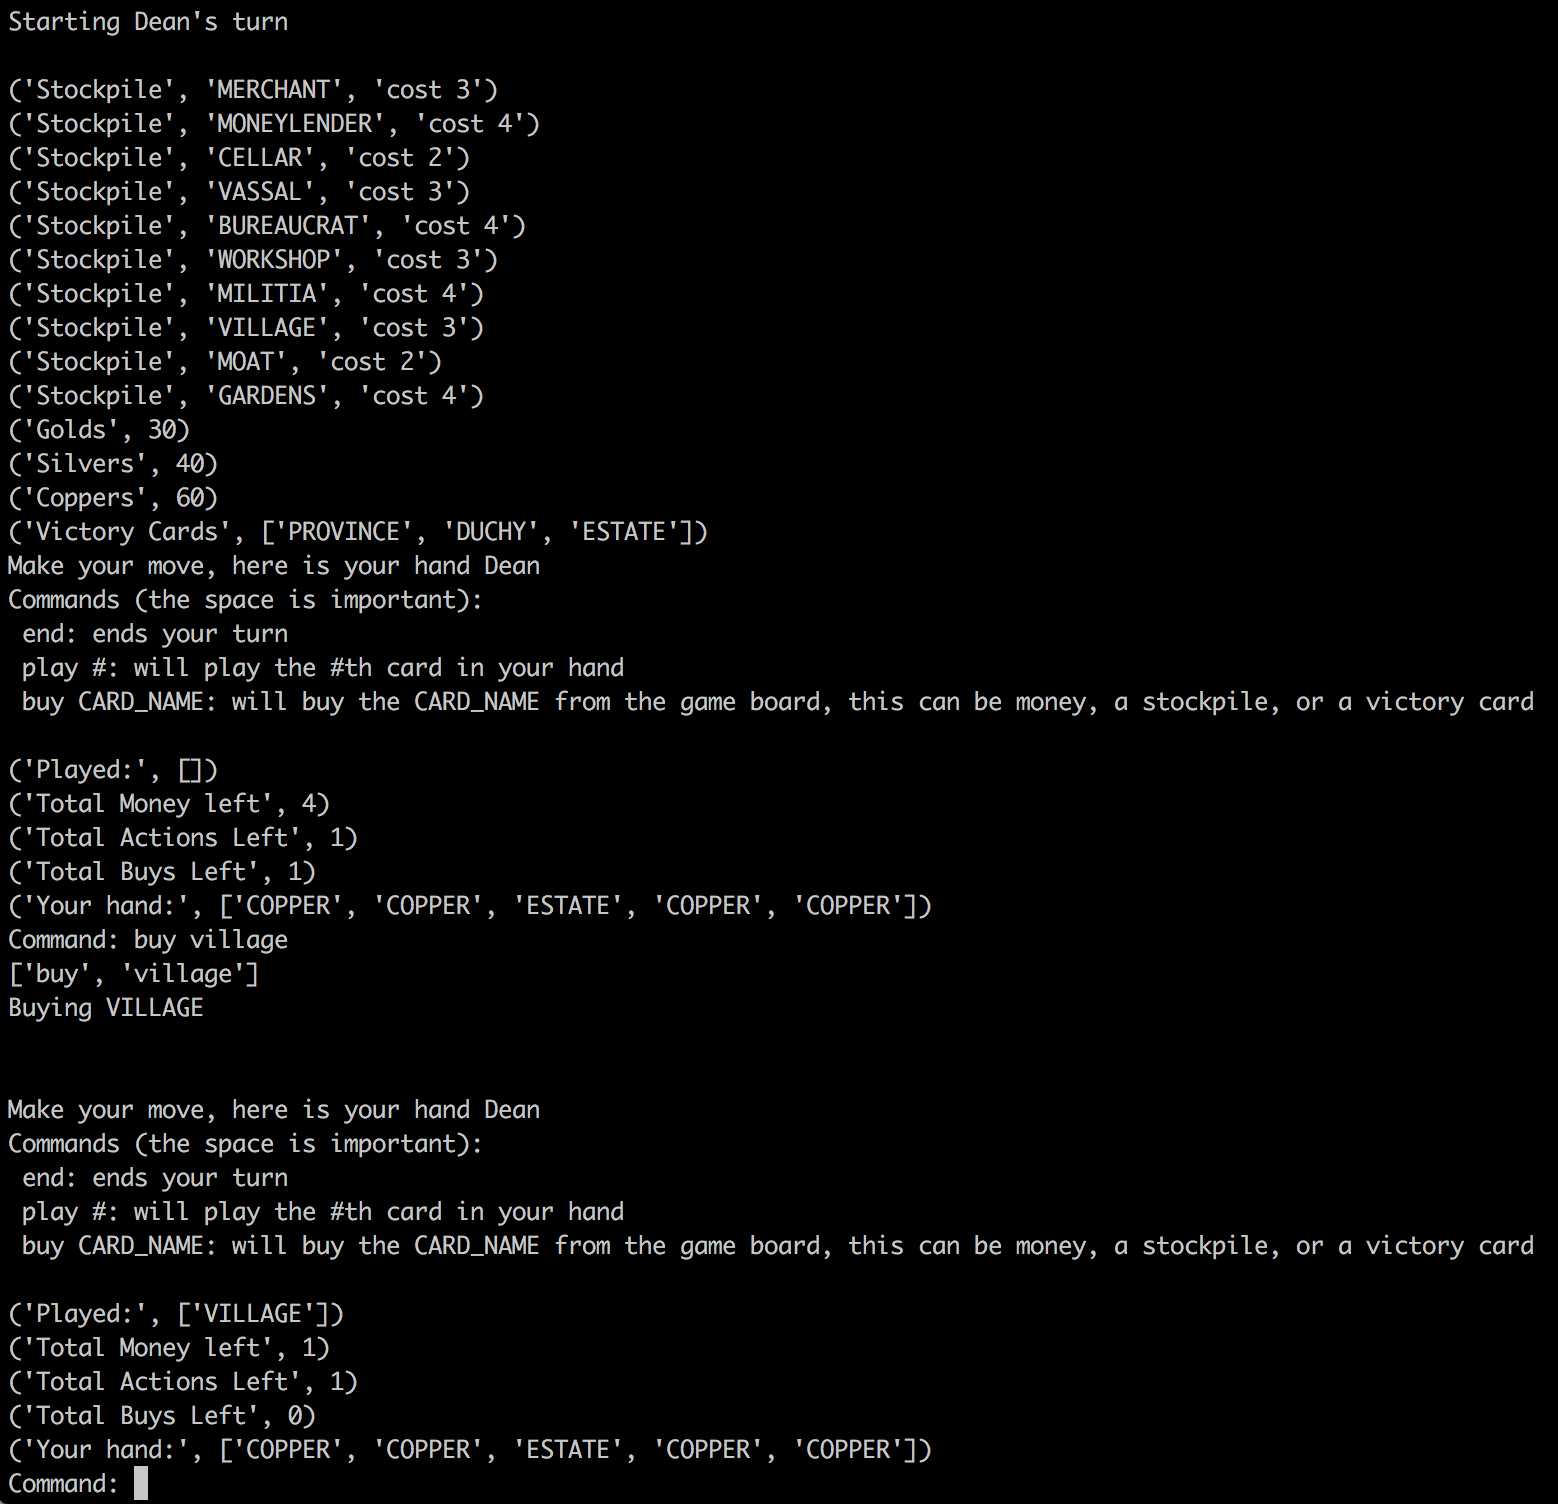
\includegraphics[width=1.5\textwidth]{commandLine}
\centering
\end{figure}


\section{Exploratory Analysis}

There are $\binom{26}{10} = 5311735$ ways to set up a game with all 26 cards. \newline
\newline
There are $\binom{12}{10} = 66$ ways with the 12 cards. This smaller test set will make things easier to analyze and break down. \newline

We know from how the deck is built and that since each player starts with 10 cards in their deck, they will go through two full hands with no actions to play. After that, assuming that player purchased an action card in the last hand, there is a 

From this, there are two approaches, I might just get a throne room, which on its own does not do anything, or the player has  X percent chance of getting a throne room and another action card. 

Another approach I took for strategy was comparing card effects to cost. For example, the village card's effects are: \begin{verbatim} +1 Card +2 Actions 3 Cost \end{verbatim}  While the Laboratory's effects are: \begin{verbatim} +2 Card +1 Actions 5 Cost \end{verbatim}
Since the only difference is the effect numbers are switches, we can conclude that buying extra cards is more valuable than extra actions. This helped design the maximum action strategies to help determine which cards should be prioritized.



\section{Strategies}

\subsection{Intuition}

There are many strategies online that talk about effective uses of different cards and different combinations that go well together. The game becomes more complicated when you potentially \textit{Throne Room} a \textit{Smithy}. Also, considering that the game is about building a hand, you want to first buy cards that help you build faster and then buy cards that give you buys/actions/money. One a good deck is built, provinces are easier to afford. 

There are two extreme strategies that should be explored in order to find a balance between the two.

	\begin{enumerate}
 		 \item Build up actions so that the player can keep playing action cards, earning more gold, and drawing more cards and hopefull more money. This extreme is useless however if no more of the cards are money. That being said, there are seven coppers total, so with the proper action cards, it is possible to buy a province. 
		 \item If a player only buys gold, then they only have 5 cards to get money, but the hope is that those cards are of higher value and will add up to at least 8. Actions would be helpful here since they might give more cards and in turn, more money. 
	\end{enumerate}
	
Obviously a balance is required between buying money and buying action cards. This is one of the objectives of this project. 


\subsection{Simulated Strategies}

These will be our data generation tools. They will record their move and in the end, record if they win or lose. As a basic rule, they 

	\begin{enumerate}
 		 \item \textbf{Random} Randomly chooses an action card if there is one and then buys a random action card that it can afford.
  		 \item \textbf{Max Actions} Takes cards that lead to more and more actions and draw cards. This might help if we learn that lots of actions builds long hands with money. 
		 \item \textbf{Max Money} Buy money whenever possible that isn't a copper. Otherwise, buy a random action
		 \item \textbf{Balance} Maintain a balance between action cards and buying money. The rationale here is give infinite actions, those don't help much if the player has no money. And vice versa, if the other player only buys money, the might lose still because only getting money might take more time. 
	\end{enumerate}

\subsection{Strategies Implemented}

For every strategy, I programmed some basic common sense heuristics into their decision making such as buying a province when that strategy has enough money and the basics rules of playing cards first before buying in order to build up money. Bellow is the structure used to add a strategy. It consists of a make and buy if statement as well as an if statement that determines the strategy to be used. This is based on the strategy name of the strategy object. See the github linked at the end of the report for more details.
\\
\\
\textbf{Make Decision Implementation with the random strategy}
\begin{verbatim}

    def make_decision(self, board):
        """
        this simply just needs to do a buy or play decision
        Generally we play actions until those are 0 or 1
        then buy depending on our strategy
        After that end turn if no buys or actions
        if they have >= 8  coins, will buy a province

        basically the simulations either choose an action or a buy
        """
        #this is true for all strategies
        buy_phase = False
        if self.my_player.buys == 0:
            self.my_player.end_turn()
            return "end"
        if self.my_player.actions == 0:
            buy_phase = True

        #self.print_board(board)
        actionable_cards = self.get_playable_cards()
        buyable = self.get_can_buy(board)
        #now strategy specific
        if self.strategy_name == "random":
            if not buy_phase:
                #time to play actions
                if len(actionable_cards) == 0:
                    self.my_player.actions = 0
                else:
                    if len(actionable_cards) == 1:
                        hand_num = actionable_cards[0]
                    else:
                        hand_num = actionable_cards[random.randint(0,
                        					len(actionable_cards) - 1)]
                    selected_card = self.my_player.hand[hand_num]
                    #print("playing " + selected_card.name)
                    try:
                        selected_card.do_action(board, self.my_player)
                        self.my_player.hand.pop(hand_num) 
                        self.my_player.played.append(selected_card)
                        self.my_player.actions -= 1
                    except Exception as e:
                        self.my_player.actions = 0
                        print(e)
                        print("cannot play that card, moving to buys instead")
            else:
                if len(buyable) == 0:
                    #no money to buy
                    self.my_player.buys = 0
                    return
                elif "PROVINCE" in buyable:
                    buy_num = buyable.index("PROVINCE")
                elif len(buyable) == 1:
                    buy_num = 0
                else:
                    buy_num = random.randint(0,len(buyable) - 1)

                choice = buyable[buy_num]
                if not board.buy(choice, self.my_player):
                    print("Unable to buy that card")
\end{verbatim}

\subsubsection{Random}

This strategy simply uses a random number generator to select a card from the available cards. I created two helper functions, \textit{get\_can\_buy} and \textit{get\_playable\_cards}, that tell the strategy what the options are. From those lists, the random number generator randomly selects a card. This includes victory cards, kingdom cards, and money piles. 

\subsubsection{Max Actions}

The cards listed bellow are the best cards for getting actions. This was determined by the number of actions that those cards give as well as pairing that with drawing cards. Drawing cards can lead to more actions, but only if that leads to another action card. SMITHY lets the player draw 3, but since they would be out of actions, it is ranked lower than cards that have draw effects and action effects. 

The strategy looks at every card in the \textit{get\_can\_buy} and \textit{get\_playable\_cards} piles, and selects the card with the lowest index in the list bellow. 

\begin{verbatim}
max_action_cards = ["LABORATORY", "FESTIVAL", "MARKET", 
		"VILLAGE", "SMITHY", "VASSAL", "MOAT"]
\end{verbatim}

\subsubsection{Max Money}

This strategy was implemented similarly to max actions, except cards that yield the most money value are first. Gold yields 3 and festival yields 2 and so on. It is worth noting that this order could be experimented with to see if the results improve. 

\begin{verbatim}
max_money_cards = ["GOLD", "SILVER", "MONEYLENDER", "FESTIVAL", "MARKET", "COPPER"]
\end{verbatim}

\subsubsection{Balance}

This strategy counts the number of cards in my hand, deck, and discard that are either part of the max\_action\_cards or the max\_money\_cards. Depending on which count is higher, the balancer will play the other strategy to try to fix the balance. For example, if the player has more max\_money\_cards, the balancer will play a max\_action\_cards strategy. 

\subsubsection{Card Specific}

Festival and Market

\subsubsection{Simplifications}

Only a subset of cards are being used for these simulations because they require no user input. The rest of the cards require some decision making beyond just picking a card to play. This isn't a big problem since the strategies can be expanded to include also decisions with other players. I am ignoring the rest of the cards however to ensure I get good results with a subset of cards. \\
\\
Copper should not be purchased, takes up one of the precious five spots in the hand. We will have random that might purchase a copper card so we will still have some player data. 

\section{Simulations}

Simulations is one of the main tools for analyzing different strategies because it allows us to play many games with varying amounts of players and strategies. From there, we can statistically say which strategy is better than the rest by running hypothesis tests on the results. To get these results, again the architecture of the game had to be modified. It was originally designed to be one game at a time, so another game mode is needed to run n numbers of games and generate win numbers from that. 

\subsection{Qualitative Insights}

Running the random tests against each other produces long games where provinces are rarely won. This makes sense because in order to get 8 money in a hand, the player either needs a string of actions or to have a lot of silver. This is much less likely if the hands are played at random. When a province is bought, we can look at which cards tend to be played that give the player enough money to buy the card. This will be useful for determining which cards give us the most value. 

Another interesting observation that comes from looking at the simulated games, the scores are higher than normal. This comes from purchasing many estates and gardens. Since the hands tend to be larger with random, the gardens have more yield because their value increases as you build up your hand.

\subsection{Win Charts}

Games were player with 3 players to start. Here is an example of some of the simulation scores: 
\\
\\
\textbf{Random} 
\\

The random strategies performed as expected. There were more outliers and the win scores were about the same. This simulation was more of pilot test to see how the simulations would interact. 

\begin{figure}[H]
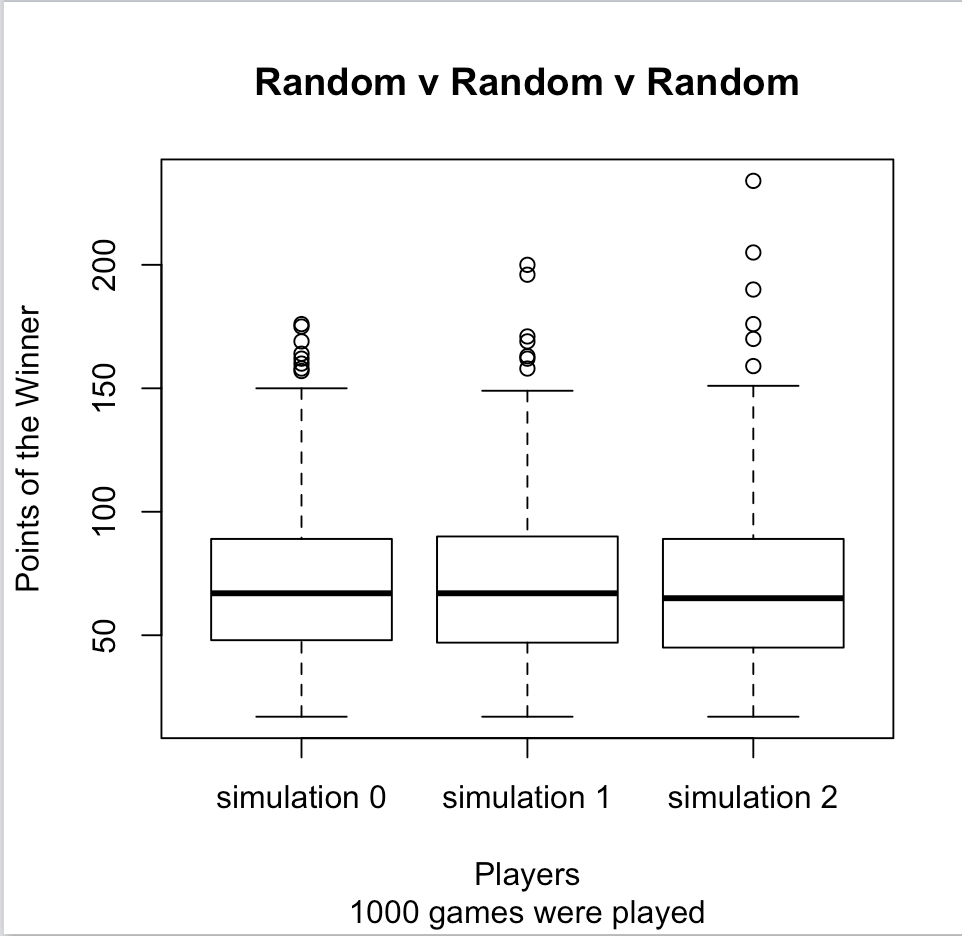
\includegraphics[width=.75\textwidth]{random_random_random}
\centering
\end{figure}

\textbf{Action vs. Money vs. Random} \\

Money strategy did the best while random rarely won. From this we have an indicator that maximizing money might be a better first strategy to get money towards buying a province. It is worth noting that the action strategy tends to lead to more cards and actions, this is effective if there is money to draw, but if only actions are drawn, then more actions are not as effective as they can be. 

\begin{figure}[H]
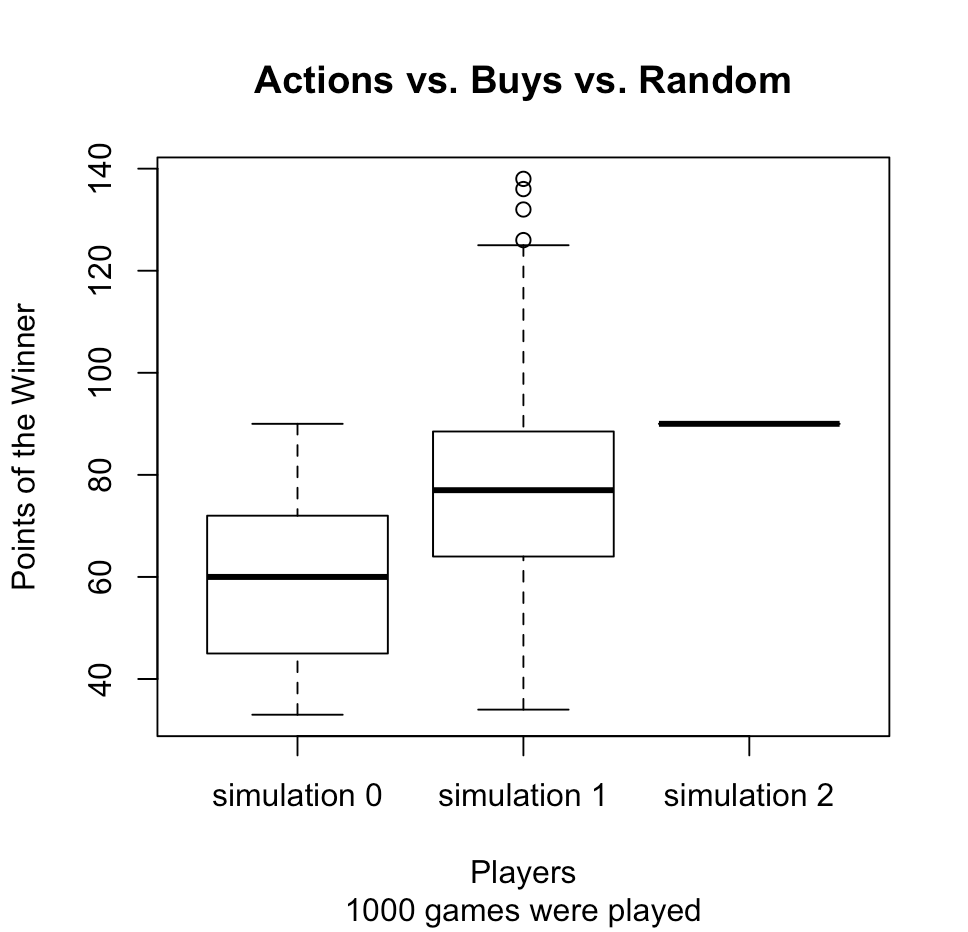
\includegraphics[width=.75\textwidth]{action_buy_random}
\centering
\end{figure}


\textbf{Balance vs. Action vs. Money vs. Random}\\

Balance takes on some of the flaws of the action strategy. Thus, it sits in-between the best strategy so far, Max Money, and the okay action strategy. 

\begin{figure}[H]
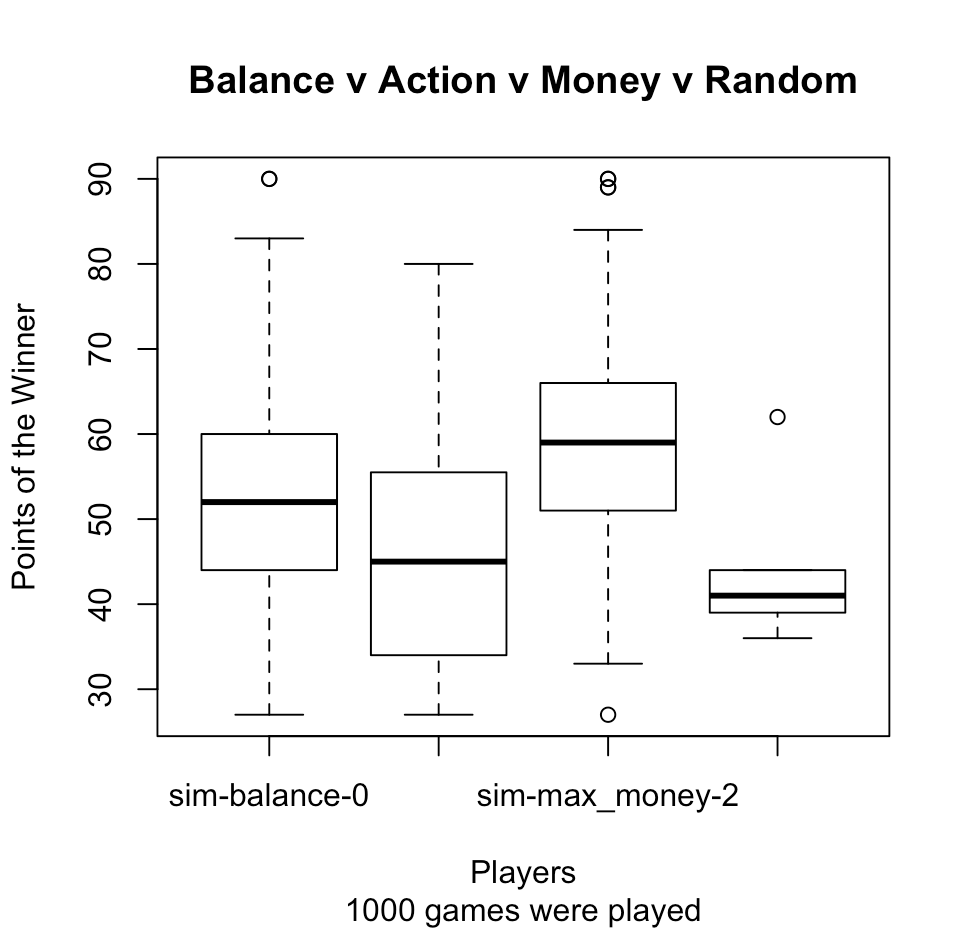
\includegraphics[width=.75\textwidth]{all_strat}
\centering
\end{figure}

\textbf{Festival vs. Market}\\

While market is slightly higher, they are similar enough that there is probably no significant difference. This will be tested in the hypothesis tests. Notice that the scores are lower for these than the other tests. Lower scores might indicate quicker wins. A quick win means someone is able to buy a province faster than normal. These cards probably work better in combination, but at least the test sheds some light that they are relatively equally balances. This indicates that their usage must depend on the situation and that by themselves, they don't differ. Their value most likely comes from working towards getting other cards. For example, getting 2 gold from festival could help push a players money count to 8 in order to purchase a Province.

\begin{figure}[H]
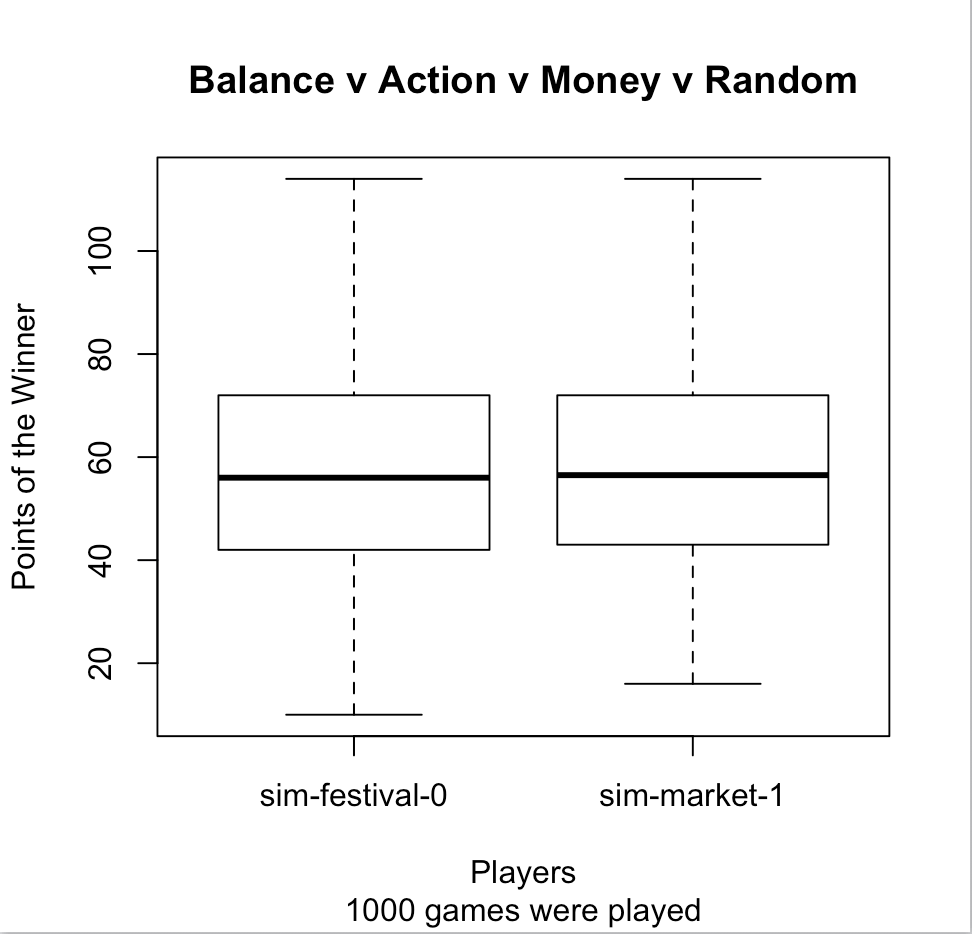
\includegraphics[width=.75\textwidth]{festival_market}
\centering
\end{figure}


Get some win results and say if they are statistically significant with some tests, get those p-values

\section{Gathering Data}

Data was stored in CSV files. For example, the random vs. random games had rows with values  $<Winner, Winner_Score>$. This entry was added to the CSV file after every simulation

Simulations were run with game parameters in one file called \textbf{\textit{commands.in}}

\begin{verbatim}
sim
1
2
3
4
5
6
7
8
9
10
random,random,random
\end{verbatim}

Then, a bash script was run to run the commands over and over again

\begin{verbatim}
#!/bin/sh
for i in `seq 1 1000`;
        do
                python play.py < commands.in
        done
\end{verbatim}


\section{Brief Model Overview}

Can talk about the models I used to for strategies

\subsection{K-Means}

\textbf{Errors}\\

\begin{center}
\begin{tabular}{||c | c ||}
\hline
 \textbf{withinss} & 8833.396 10936.840 24079.819 14742.027 \\ 
 \textbf{betweenss} & 192660.3 \\  
 \hline
\end{tabular}
\end{center}

\begin{figure}[H] \centering
   \begin{minipage}{0.49\textwidth}
     \frame{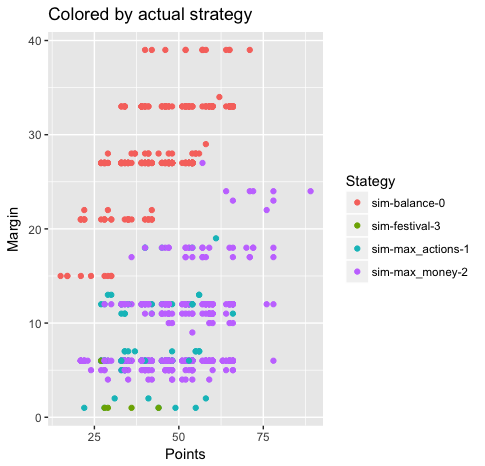
\includegraphics[width=\linewidth]{actual_points}}
   \end{minipage}
   \begin {minipage}{0.49\textwidth}
     \frame{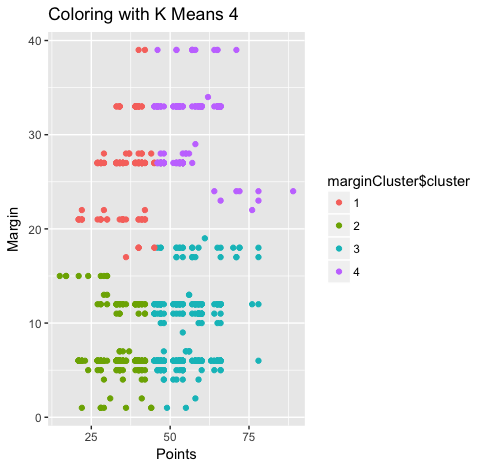
\includegraphics[width=\linewidth]{kmeans}}
   \end{minipage}
\end{figure}

\subsection{Hypothesis Testing}

Using hypothesis tests, we can now answers questions like, 'Is playing festival on average a better move than market?' or 'Is strategy A, on average, better than strategy B?'

\begin{verbatim}
#now strategy differences
colnames(win_all) <- c("Name", "Points")
money_v_random = win_all[(win_all$Name == "sim-max_money-2" | 
		win_all$Name == "sim-random-3"), ]

counts = c()
for (item in money_v_random$Name) {
  if (item == "sim-max_money-2") {
    counts = c(counts, 1)
  } else {
    counts = c(counts, 0)
  }
}
money_v_random$counts = counts
money_v_random$Name <- droplevels(money_v_random$Name)
prop.test(table(money_v_random$counts, money_v_random$Name), correct = FALSE)
\end{verbatim}

\subsubsection{Results}

\begin{figure}[H] \centering
   \begin{minipage}{0.49\textwidth}
     \frame{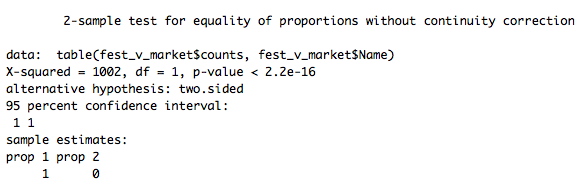
\includegraphics[width=\linewidth]{mark_fest_test}}
   \end{minipage}
   \begin {minipage}{0.49\textwidth}
     \frame{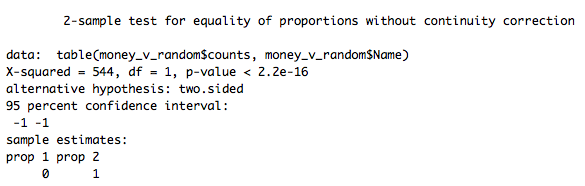
\includegraphics[width=\linewidth]{mon_rand_test}}
   \end{minipage}
\end{figure}

\section{Risks}

Strategies don't produce good results for testing because having the entire game come down to just just one win/loss classification doesn't make realistic sense for scaling this approach. Every move could be taken into consideration for more accurate results. There would need to be a way to measure if each move is good or bad though. 
\\
The action strategy might not be good because it could be more of a support role, meaning it works well in combination to other cards, but not by itself against a money strategy. This also accounts for the weaknesses in balance. To fix this, strategies need to be smarter with more rules to discover these additional benefits from pairing action cards. Money cards don't pair well which makes a direct comparison harder. 
\\
Not testing more of the cards, but would make the simulations much more complicated. This was still a good approach for understanding the relationship between drawing, buying money, and buying cards that give actions.

\section{Results}

\section{Summary}

\section{Coding Reflection}

	\begin{enumerate}
 		 \item Testing framework should be part of the design upfront. I had to test most things manually which was not as efficient as it could have been and it doesn't let me catch as many bugs. What was useful was simulations which caught a lot of errors. 
	\end{enumerate}



\section{Miscellaneous and further ideas}

There are many different approaches to analyzing this game and many more questions that could have been asked. Throughout the process, I wrote down different aspects of the game that could have been tested. Here are some of the things that could be done on top of what I already did. Since the game can be easily adapted to include other modes of play and other simulations, they are not difficult to add on. \\

One thing to look at is getting more information out of each simulation, right now the outputs are only who wins and the points that were scored by the winner. However, other good information might be things such as typo of victory (either based on the stockpiles or provinces) and margin of victory. These numbers could be used to figure out a ranking of scores. So this way instead of having to run a lot of simulations with different strategies, instead one could find scores of how well the simulations perform. This might help quantify how good specific modifications are to strategies. 
\\
\\
\textbf{Additional modes:}\\
A game helper mode would make all of this information practical. It would take in information about a game someone is playing and recommend a move for them. This would be useful for putting the project insights to the test by actually providing insights into a particular game. Another mode would be person versus computer strategy mode where individuals can play against their strategies. 
\\
\\
\textbf{Additional Strategies:}\\
There are many more strategies that can be tried to find the best solution. We could run a simulation to see if Village is better than Cellar. This is fun for answering simple queries like "is card x better than card y," but to really figure out more into an optimal strategy, we need to do more machine learning to figure out our best moves. 
\\
\\
\textbf{Additional things to explore time permitting:}\\
	\begin{enumerate}
 		 \item Average score for each simulation
		 \item Probability of particular hands to help guide the strategies
		 \item more simulations
		 \item probability models
		 \item Incorporate ML concepts  to Dominion, the goal is to maximize points and we would train on the moves in a game that lead to increased points only if that game leads to a win
		 \item Redesign the game in some aspects, making the game modes more modular and the simulations easier to adjust
		 \item Program more cards to auto play so simulations still work
	\end{enumerate}
	

TO ADD
based on the cost of village and lab, I said cards are more valuable than actions if they are both present (smitty)

how I designed the strategies, actions vs money and always buying a province. How the base should be better than random but its a good first thing. 

make it so each strategy buys a province if they can and redo your simulations!

check this doc with Grammarly - test run


\section{Open Source}

I wanted to make sure all the code can be viewed and experimented with. My github can be found here: \url{https://github.com/rollonbears234/dominion-game}. 



%\subsection{}
\end{document}
